%\section{RADS Approach To Anomaly Detection}
\section{RADS Window-based Time-series Analysis}
\label{sec:approach}
\noindent 
%From the previous section, we observe an important point that the standard deviation resulted from the genuine workload spikes is significantly higher than the other standard deviation values. 
%This can be used as an indicator for the genuine workload spikes to not identify them as anomalies. 
%Based on this we propose a new approach to differentiate the anomalous behaviour due to attack from the normal behaviour. Our approach uses a combination of the volume (average) and the underlying distribution (standard deviation) of the raw data. 
%In this section we propose a new approach to differentiate a Cloud VM's ``anomalous" behaviour from its ``normal" behaviour. 
%The novelty of the approach lies in its ability to classify genuine Cloud workload spikes as ``normal" in order to remove false positives arising due to wrongly classifying spikes as ``anomalies".
%In this section we propose RADS approach to detect anomalies in the Cloud data centres. The key idea of this approach is to differentiate the genuine Cloud workload spikes from the “anomalies” in order to identify them as “normal” and remove false positives without compromising the accuracy of anomaly detection. This is achieved by considering the combination of the average and the standard deviation of the raw data. The idea stems from the following important observation from the previous section: average value of raw data measured during the workload spike situation is higher than the average values measured during the normal situation, which is accompanied by a very high standard deviation value (higher than the standard deviation values measured during the normal and the anomalous situations).
%In this section we propose RADS approach to detect anomalies in the Cloud data centres. 
%The novelty of this approach is its ability to differentiate the genuine Cloud workload spikes from the anomalies in order to reduce false positives without compromising the accuracy of anomaly detection. 
%To achieve this, RADS uses a window-based time series analysis which combines average and standard deviation of the raw data in each time series window; and uses artificial data points that represent workload spikes. 
%The idea stems from the following important observation from the previous section: 
%average value of raw data measured during the workload spike situation is higher than the average values measured during the normal situation, which is accompanied by a very high standard deviation value (higher than the standard deviation values measured during the normal and the anomalous situations). 
%This is achieved by considering the combination of the average and the standard deviation of the raw data. The idea stems from the following important observation from the previous section: \textit{average value of raw data measured during the workload spike situation is higher than the average values measured during the normal situation, which is accompanied by a very high standard deviation value (higher than the standard deviation values measured during the normal and the anomalous situations). }
%The novelty of the approach lies in its ability to classify between anomalies and genuine Cloud workload spikes in order to remove false positives arising due to wrongly identifying spikes as ``anomalies".
%The approach uses combination of the volume (average) and the underlying distribution (standard deviation) of the raw data. 
%The approach uses combination of the average and the standard deviation of the raw data. 
%COMBINATION OF AVG AND SD GRAPH
%\vfill
\begin{figure}[!h]
  %\vspace{-0.2cm}
  \centering
   {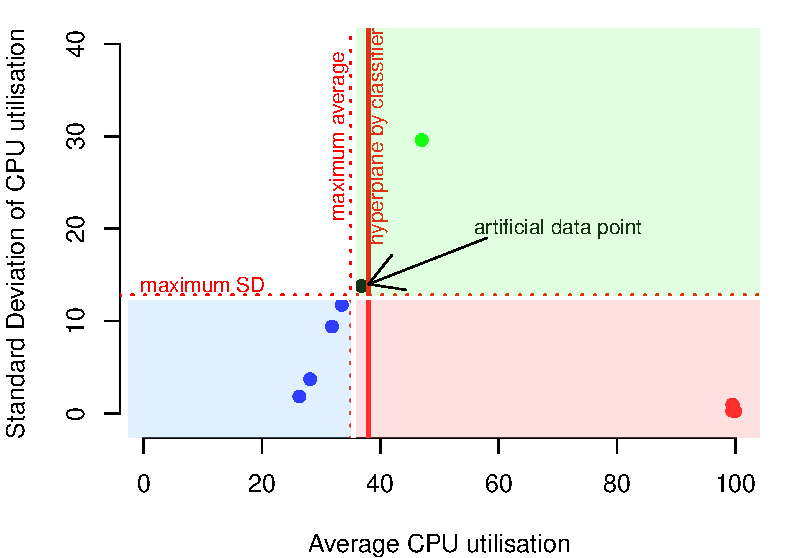
\epsfig{file = figures/approach_avg_sd_dot, width = 0.8\columnwidth}}
   \caption{RADS approach: combining average and standard deviation}
  \label{fig:avg_sd_combined}
  %\vspace{-0.1cm}
\end{figure}
%\vfill

\noindent In this section we explain RADS window-based time series analysis that resolves the problems identified in the previous section. 
%The novelty of this approach is its ability to differentiate the genuine Cloud workload spikes from the anomalies in order to reduce false positives without compromising the accuracy of anomaly detection. 
Specifically, RADS combines average and standard deviation of the raw data in each time series window; and uses artificial data points that represent workload spikes. 

If we combine the average and standard deviation values generated from the experiment as discussed in the previous section, then we can represent them in a two-dimensional space as shown in Figure~\ref{fig:avg_sd_combined}. Similar to the previous section, blue, red, and green dots refer to the measurements during the normal, anomalous, and spike situations, respectively. From the figure we observe that the coloured dots can be classified into three classes if we draw the dotted red hyperplanes (horizontal and vertical) based on the maximum average on x-axis and maximum standard deviation (SD) on y-axis. Hence, this becomes a three class classification problem, where the classes can be labeled as: ``normal'' (blue coloured section) containing blue dots, ``anomaly'' (pink coloured section) containing red dots, and ``spike'' (green coloured section) containing green dot. However, we do not wish to go in that direction of classification as we assume that the samples for the ``anomaly'' class as well for the ``spike'' class are not available or known. 
%\textbf{RADS window-based time-series analysis:} 
%Figure~\ref{fig:avg_sd_combined} presents coloured dots in a two-dimensional space to represent both average and standard deviation values of the CPU utilisation (collected from the experiment discussed in the previous section). Similar to the previous section, blue, red, and green dots refer to the measurements during the normal, anomalous, and spike situations, respectively. 
%demonstrates how the approach helps in solving the problems identified in the previous section. 
%From the figure we observe that the coloured dots can be classified into three classes if we draw the dotted red hyperplanes (horizontal and vertical) based on the maximum average on x-axis and maximum standard deviation (SD) on y-axis. Hence, this becomes a three class classification problem, where the classes can be labeled as: ``normal'' containing blue dots, ``anomaly'' containing red dots, and ``spike'' containing green dot. However, we do not wish to go in that direction of classification as we assume that the samples for the ``anomaly'' class as well for the ``spike'' class are not available or known. 
%Figure~\ref{fig:avg_sd_combined} demonstrates how the approach helps in solving the problems identified in the previous section. From the figure we observe that the blue, red, and green dots can be classified into three classes if we draw the dotted red hyperplanes (horizontal and vertical) based on the maximum average on x-axis and maximum standard deviation (SD) on y-axis. Hence, this becomes a three class classification problem, where the classes can be labeled as: ``normal'' for blue dots, ``anomaly'' for red dots, and ``spike'' for green dot. However, we do not wish to go in that direction of classification as we assume that the samples for the ``anomaly'' class as well for the ``spike'' class are not available or known. 
%To handle this classification problem we combine the following approaches together:
%To resolve this classification problem we consider the following steps:

%To convert the three class classification problem into two class classification problem, we consider using artificial data points representing genuine workload spikes.
%\begin{enumerate}[{(1)}]
%\item \textit{Use of artificial data points for representing genuine workload spikes:}
%This step converts the three class classification problem into two class classification problem.  
%As mentioned in the previous section, we consider that the anomalies (red dots) and the genuine workload spikes (green dot) are appearing only during the testing or detection phase of the classifier. Therefore, 
%If genuine workload spikes (the green dot) occur during the training phase of the OCC algorithm, they can be recorded as ``normal" in order to include the ``spike" class within the ``normal'' class. Hence, step (1) will suffice for a successful classification of the ``anomaly" class in that case. 
%As we assume that the genuine workload spikes are not seen during the training phase, we need to use artificial data points for representing the genuine workload spikes which can appear during the testing or the detection phase, so that the OCC algorithm classifies them as ``normal".
%We consider the latter condition in our experimental evaluation and therefore, 
%\textcolor{red}{We consider the latter condition and therefore, in this step 
RADS represents the green dot (``spike" class) with an artificial data point (black dot) which is a vector of the form: (max\_avg, max\_SD), where the max\_avg and the max\_SD are the maximum average and standard deviation of the blue dots (``normal'' class), respectively. This representation is based on the following assumptions: 
%Importantly, considering the assumptions we can differentiate the ``spikes" from the ``anomalous" behaviour. 

\begin{itemize} %[{(1)}] 
\item \textbf{Assumption-3:} Workload spikes exhibit average and standard deviation values higher than the maximum average and standard deviation values exhibited by ``normal" behaviour, respectively. That means that in Figure~\ref{fig:avg_sd_combined}, the assumption is that the green dot will never reside in the pink coloured section. 
\item \textbf{Assumption-4:} Anomalies exhibit standard deviation values lower than the maximum standard deviation value exhibited by ``normal" behaviour. That means that in Figure~\ref{fig:avg_sd_combined}, the assumption is that the red dots will never reside in the green coloured section. 
%\item \textbf{Assumption-3:} Workload spikes exhibit average values higher than that exhibited by ``normal" behaviour and they exhibit standard deviation values higher than that exhibited by both ``normal" and ``anomalous" behaviour. 
%which can be captured as anomaly by the machine learning or statistical approaches. 
\end{itemize}  %[{(1)}] }

%We can see an evidence of these assumptions in Figure~\ref{fig:avg_sd_combined}.  
We define the workload spikes as high utilisation values which persist only for a momentary period of time. Hence, in a time series window, the spikes will generate a high average value with a high standard deviation value and this will support Assumption-3.
We can support Assumption-4 with the fact that due to the nature of their attack, both DDoS and cryptomining attacks consume the resources significantly in a consistent manner without interrupt, whereas, resource consumption in a ``normal" behaviour is expected to have inconsistency and interruption. 

Thus, using the artificial data point RADS converts the three class classification problem into a two class classification problem where the classes are now: (i) ``positive'', which is composed of known ``normal" (blue dots) and unknown ``spike" (black dot) samples and (ii) ``negative'', which is composed of unknown ``anomaly" (red dots) samples. 
In Figure \ref{fig:avg_sd_combined} we can see that the two classes are clearly separable by a solid red hyperplane. Hence, a linear classifier can successfully differentiate between the two classes and produce high accuracy with low false positives. 
%As we assume that the samples for the “negative” class are unknown, to differentiate between the two classes, RADS uses OCC algorithm that is proposed by Hempstalk et al. in~\cite{OCC:2008}. 
%The algorithm first generates the artificial data (the red dots belonging to the ``negative" class) from a multi-variate normal distribution as estimated from the training data (the blue dots belonging to the ``positive'' class) and second, uses these artificial data as a second class in the construction of a binary class classification model, which is capable of classifying between the `positive'' and the ``negative'' class. 
%Thus, this approach requires training with the data belonging to the ``normal" class in order to build the OCC models, which can classify between the `normal'' and the ``anomaly'' class. 
%The classification is based on Bayes' Theorem\footnote{http://www.investopedia.com/terms/b/bayes-theorem.asp}.}

%Hence, RADS can successfully differentiate between the ``normal" and the ``anomalous" behaviour. 
%Importantly, RADS can differentiate between the ``spikes" and the ``anomalous" behaviour and remove the false positives occuring due to wrongly identifying them as ``anomalies". 
%Importantly, RADS can consider the genuine Cloud workload spikes as ``normal" and remove the false positives occurring due to wrongly identifying them as ``anomalies". 

%\item \textit{Use of One Class Classification (OCC) algorithm:} 
%This step uses the OCC algorithm that is proposed by Hempstalk et al. in~\cite{OCC:2008}. 
%This step solves the two class classification problem using OCC algorithm that is proposed by Hempstalk et al. in~\cite{OCC:2008}. 
%The algorithm first generates the artificial data (the red dots belonging to the ``anomaly" class) from a multi-variate normal distribution as estimated from the training data (the blue dots belonging to the ``normal'' class) and second, uses these artificial data as a second class in the construction of a binary class classification model, which is capable of classifying between the `normal'' and the ``anomaly'' class. 
%Thus, this approach requires training with the data belonging to the ``normal" class in order to build the OCC models, which can classify between the `normal'' and the ``anomaly'' class. 
%The classification is based on Bayes' Theorem\footnote{http://www.investopedia.com/terms/b/bayes-theorem.asp}.

%We observe from Figure~\ref{fig:avg_sd_combined} that the genuine workload spikes generate the average and standard deviation values, which are higher than the maximum average (max\_avg) and standard deviation (max\_SD) values, respectively, generated by the blue dots (``normal'' class). 
%Therefore, we use the artificial data points (``black" dot) as vectors of the form: (max\_avg, max\_SD). 
% to consider them as ``normal". 
%In case the genuine workload spikes are occurring during the training phase then using only approach (a) will suffice as in that case, the spike samples can be recorded as ``normal" by OCC algorithm. But, if the genuine workload spikes are not seen during the training phase and they are only appearing during the testing or the detection phase then we need to use both approach a and b. We consider the latter condition in our experimental evaluation.
%Similarly, during the detection process, this approach represents the test sample containing genuine workload spikes with an artificial data point so that the OCC model classifies that as ``normal". 
%This helps the OCC models to classify the genuine workload spikes occurring during the detection process as ``normal". 
%We observe from Figure~\ref{fig:avg_sd_combined} that the genuine workload spikes generate the average and standard deviation values, which are higher than the maximum average (max\_avg) and standard deviation (max\_SD) values, respectively, generated by the blue dots (``normal'' class). 
%Therefore, we use the artificial data points (``black" dot) as vectors of the form: (max\_avg, max\_SD). 
%Therefore, during the training of the OCC models, we use the artificial data points as vectors of form: (max\_avg, max\_SD). Whereas, during the detection process, we firstly identify whether the test sample contains genuine workload spikes, which we achieve by checking if the average and standard deviation values during the detection period are higher than max\_avg and max\_SD respectively, and secondly, if the the test sample contains genuine workload spikes, we use an artificial data point as a vector of form: (max\_avg, max\_SD) to represent the test sample. }
%Therefore, to generate the artificial data points during the training of the OCC models, we use the maximum average and standard deviation measured from the raw training data set (the blue dots). To generate the artificial data point}
%We measure the maximum average and standard deviation from the raw training data set (the blue dots, i.e. the ``normal'' class) and use them to create the artificial data points (the black dot) which are vectors of form $\big[maximum\_average, maximum\_sd\big]$. }
%These artificial data points are then fed to the classification model labelled as ``normal''.}
%These artificial data points are then fed to the classification model labelled as ``normal''.}
%\end{enumerate}
%Important to note that the instantaneous spikes are considered to be arising during the testing or the detection phase and not during the training phase of a classification. 

%Overall, using the steps (1) and (2) we transform the three class classification problem into a two class classification problem where the classes are now: (i) ``positive'', which is composed of known ``normal" (blue dots) and unknown ``spike" (black dot) samples; in the figure we can see them surrounded by the solid red hyperplanes and (ii) ``negative'', which is composed of unknown ``anomaly" (red dots) samples; in the figure we can see them separated by the hyperplane. 
%Overall, using the steps (1) and (2) we transform the three class classification problem into a two class classification problem where the classes are now: (i) ``positive'', which is composed of known ``normal" (blue dots) and unknown ``spike" (black dot) samples and (ii) ``negative'', which is composed of unknown ``anomaly" (red dots) samples. 
%In Figure \ref{fig:avg_sd_combined} we can see that the two classes are separable by a solid red hyperplane.
%Hence, RADS can successfully differentiate between the ``normal" and the ``anomalous" behaviour. 
%Importantly, RADS can differentiate between the ``spikes" and the ``anomalous" behaviour and remove the false positives occuring due to wrongly identifying them as ``anomalies". 
%Importantly, RADS can consider the genuine Cloud workload spikes as ``normal" and remove the false positives occurring due to wrongly identifying them as ``anomalies". 

Similar to the CPU utilisation pattern deviation due to cryptomining attack, network traffic pattern deviates significantly due to DDoS attack. This is observed in~\cite{ddso_charater_2017} where they analysed DDoS attack samples taken from the CAIDA\footnote{http://www.caida.org/data/passive/ddos-20070804\_dataset.xml} dataset. Therefore, RADS analyses network traffic behaviour in the exactly the same manner as CPU utilisation behaviour analysis (discussed in this section) in order to detect VM-level anomalies occurring due to DDoS attack.

VMs may host varieties of applications in a Cloud data centre, some of which may be CPU intensive, some may be network intensive, and some may be both CPU and network intensive. Analysing both the CPU and network behaviour together makes the raw data points two dimensional, where in many cases one of the two parameters of the data points may generate steady time series data without any variance. In such cases, classification algorithms may suffer from the curse of dimensionality. We experimentally found this happening while executing two different Cloud applications (one CPU intensive and another network intensive) in our testbed. Therefore, RADS analyses the CPU and the network behaviour separately although it can perform both in parallel if required. 

%We collect the known normal samples as the training data samples from running the cloud applications on the cloud data centre. The unknown anomaly and spike samples are generated by approach a and b respectively. 
%Importantly, if we consider that the genuine workload spikes are occurring during the training phase then using only approach a will suffice as in that case, the spike samples can be recorded as normal by OCC algorithm. But, if we consider that the genuine workload spikes are not seen during the training phase and they are only appearing during the testing or the detection phase then we need to use both approach a and b. We consider the latter condition in our experimental evaluation.
%~\cite{OCC:2008} experimentally proved that the OCC algorithm (used by approach (a)) achieves better performance than the one-class Support Vector Machine (SVM) algorithm (used by Watson et al. in~\cite{cloud-malware:2016}). 
%Step (2) is based on the \textbf{assumption}: \textit{genuine workload spikes during a Cloud application's ``normal" behaviour produce high average values (higher than the other average values observed in the ``normal" data), which are accompanied by very high standard deviation values (higher than the standard deviation values observed in the ``normal" and the ``anomalous" data).} 
%We have seen some proof of this assumption in the previous section and we support this further in Section~\ref{sec:experiments} with further experiments. 
%We have seen proof of this assumption in the previous section. 
%We design a new algorithm for RAIDS based on the approaches a and b, which we explain in Section~\ref{sec:algorithm}. We also provide experimental proofs on the validity and the performance of the approaches in Section~\ref{sec:experiments}.
